%!TEX ROOT = thesis.tex

\chapter{Semantics Retrieval Engine}

\label{section:retrievalengine}
\section{Introduction}

As described in Section \ref{section:introduction}, there's an evident gap between the process of obtaining user described events and the retrieval of the intended video shots. Traditional approach of collecting text-based description of events alone are insufficient for effective retrieval process.  With the vehicle-specific features such as the vehicle trajectory, time-stamp information, and color information extracted via the extraction module introduced in Chapter \ref{section:semanticsextraction}, retrieval modules were designed to retrieve video shots that resembles user described queries. This chapter aims to engage the topic of semantic retrieval engines in detail and evaluate their performances along with analysis of the end results.


In this chapter, two retrieval module with relatively different concepts and underlying framework are discussed. The first module was designed with a classic document retrieval system in mind, while the second module was developed in order to address the shortcomings of the first. This is then followed by the methods used to measure the difference between the user-described trajectory, methods used to classify the vehicle color, scoring system along with the results based on multiple user's review of the proposed method. This chapter also includes the speed measurement of the second retrieval engine.


\cc{please measure the VISER retrieval speed and attach the results.}




\section{\versionOne}
This section uncovers the techniques used behind this retrieval engine's framework along with the results. As previously introduced, as this retrieval engine was inspired by Locality Sensitive Hashing (LSH), documents are hashed into similar locations depending on the similarity. With that in mind, first, the concept of this retrieval engine is discussed. Next, the scoring system is discussed, the evaluation of the system is performed and recorded in the following subsections.




\subsection{Concept}
By taking advantage of the spatio-temporal atom cubes structure introduced in Chapter \ref{section:atoms}, each cataloged event in an atom were treated as an unique document. The underlying atom-based structure allows queries to be formed in a way which emulates the semantics extraction process, hence, eliminating the need for query parsing which in turn reduces the need of both pre- and post-processing of the given queries. 

In this setup, each document that contains similar contents were placed in the same SQL table as a mode of clustering documents. An example is given in Table \ref{table:dbSample} to provide a better visualization of the proposed method. These sequence of events is also visualized in Figure \ref{fig:motionExample} with the trajectory marked with \textcircled{2}. In the example, a red vehicle was detected frame 180 to 184 of a video file on the 19th of March 2016 at 8:51:00am until 8:51:05am, from atom location (3,15) to (5,17) but was detected as a pink vehicle at frame 181. Using Equation \ref{eq:file_timing}, the event's current frame time can be calculated. Given that the current frame is 181, the current frame time would equate to  $(6_{minutes} \times \frac{181}{360}) + 08:48:00am = 8:51:01am$.

As each cataloged event is treated as a unique document (a single record in the database) in this framework, the retrieval process begins by filtering out tables which are irrelevant to the query, $\mathbb{Q}$. Falling back on the example given in Table \ref{table:dbSample}, the system is able to effectively skip through 9 color tables and 5 motion tables, hence speeding up the process to locate documents of interest while reducing the overhead cost involved when going through an entire database. Upon filtering out irrelevant tables, the retrieval engine proceeds to extract and group all the relevant records according to the filenames.

Next, the retrieved results are validated to see if they belong to the same vehicle by cross-checking the obj\_id, along with that, the retrieval engine also performs validation to check if the results belong to a similar time-frame by comparing the t-coordinate. This step is essential to ensure that the results belong to the same vehicle trajectory group as the initial tracker may re-assign a obj\_id to another vehicle during the background subtraction process. While the results returned at this point were accurate, one major problem that occurs using the current process is the low recall rate. The recall rate in a retrieval engine can be thought as the percentage of relevant documents which were retrieved over the total amount of relevant documents; while a low recall rate is preferable in an environment where the accuracy of the retrieved result is regarded with high importance and false negatives are welcomed over false positive such as the medical industry, this was not the case in the proposed method.

In order to overcome the limitation of the low recall rate, a Confidence Value (CV) score parameter was introduced. The CV parameter was used to adjust the sensitivity level of accepting a video shot as part of the final retrieved results. In the proposed method, a lower CV would return a larger set of results at the expense of an increase of retrieved shots which may or may not improve the overall accuracy of the retrieval engine. Each retrieved shot, $\mathbb{S}_i$, will be accepted as the final retrieved results if it fulfills the condition in Equation \ref{eq:CVscore}. The use of the CV score parameter provides a margin of error when performing the query which acts as a trade-off function.

\begin{equation}
\label{eq:CVscore}
CV < \frac{\text{length}(\mathbb{S}_i)}{\text{length}(\mathbb{Q})} \times 100\%
\end{equation}



Upon validating the sanctity of the results, commands were sent to FFmpeg to extract the video shots based on the given filename along with the start and end frame number. Finally, the users are presented with the output from the retrieval engine where the final results can be viewed.


% Please add the following required packages to your document preamble:
% \usepackage[normalem]{ulem}
\begin{table}[hbt]
	\centering 
\caption{Database structure for a vehicle identified as red and pink color with object id "1" of the \versionOne }
\label{table:dbSample}
\begin{tabular}{llllll}
\multicolumn{6}{l}{{ color\_red}} \\ \hline
\multicolumn{1}{|l|}{\textbf{row\_id}} & \multicolumn{1}{l|}{\textbf{filename}}    & \multicolumn{1}{l|}{\textbf{obj\_id}} & \multicolumn{1}{l|}{\textbf{atom\_x}} & \multicolumn{1}{l|}{\textbf{atom\_y}} & \multicolumn{1}{l|}{\textbf{atom\_t}} \\ \hline
\multicolumn{1}{|l|}{n}                & \multicolumn{1}{l|}{20160319\_084800.mp4} & \multicolumn{1}{l|}{1}                & \multicolumn{1}{l|}{3}                & \multicolumn{1}{l|}{15}               & \multicolumn{1}{l|}{180}              \\ \hline
\multicolumn{1}{|l|}{n+1}              & \multicolumn{1}{l|}{20160319\_084800.mp4} & \multicolumn{1}{l|}{1}                & \multicolumn{1}{l|}{3}                & \multicolumn{1}{l|}{16}               & \multicolumn{1}{l|}{182}              \\ \hline
\multicolumn{1}{|l|}{n+2}              & \multicolumn{1}{l|}{20160319\_084800.mp4} & \multicolumn{1}{l|}{1}                & \multicolumn{1}{l|}{4}                & \multicolumn{1}{l|}{16}               & \multicolumn{1}{l|}{183}              \\ \hline
\multicolumn{1}{|l|}{n+3}              & \multicolumn{1}{l|}{20160319\_084800.mp4} & \multicolumn{1}{l|}{1}                & \multicolumn{1}{l|}{5}                & \multicolumn{1}{l|}{17}               & \multicolumn{1}{l|}{184}              \\ \hline
                                       &                                           &                                       &                                       &                                       &                                       \\
\multicolumn{6}{l}{{ color\_pink}}                                                                                                                                                                                                              \\ \hline
\multicolumn{1}{|l|}{\textbf{row\_id}} & \multicolumn{1}{l|}{\textbf{filename}}    & \multicolumn{1}{l|}{\textbf{obj\_id}} & \multicolumn{1}{l|}{\textbf{atom\_x}} & \multicolumn{1}{l|}{\textbf{atom\_y}} & \multicolumn{1}{l|}{\textbf{atom\_t}} \\ \hline
\multicolumn{1}{|l|}{m}                & \multicolumn{1}{l|}{20160319\_084800.mp4} & \multicolumn{1}{l|}{1}                & \multicolumn{1}{l|}{3}                & \multicolumn{1}{l|}{16}               & \multicolumn{1}{l|}{181}              \\ \hline
                                       &                                           &                                       &                                       &                                       &                                       \\
\multicolumn{6}{l}{{ direction\_down}}                                                                                                                                                                                                          \\ \hline
\multicolumn{1}{|l|}{\textbf{row\_id}} & \multicolumn{1}{l|}{\textbf{filename}}    & \multicolumn{1}{l|}{\textbf{obj\_id}} & \multicolumn{1}{l|}{\textbf{atom\_x}} & \multicolumn{1}{l|}{\textbf{atom\_y}} & \multicolumn{1}{l|}{\textbf{atom\_t}} \\ \hline
\multicolumn{1}{|l|}{h}                & \multicolumn{1}{l|}{20160319\_084800.mp4} & \multicolumn{1}{l|}{1}                & \multicolumn{1}{l|}{3}                & \multicolumn{1}{l|}{15}               & \multicolumn{1}{l|}{181}              \\ \hline
                                       &                                           &                                       &                                       &                                       &                                       \\
\multicolumn{6}{l}{{ direction\_motionless}}                                                                                                                                                                                                    \\ \hline
\multicolumn{1}{|l|}{\textbf{row\_id}} & \multicolumn{1}{l|}{\textbf{filename}}    & \multicolumn{1}{l|}{\textbf{obj\_id}} & \multicolumn{1}{l|}{\textbf{atom\_x}} & \multicolumn{1}{l|}{\textbf{atom\_y}} & \multicolumn{1}{l|}{\textbf{atom\_t}} \\ \hline
\multicolumn{1}{|l|}{j}                & \multicolumn{1}{l|}{20160319\_084800.mp4} & \multicolumn{1}{l|}{1}                & \multicolumn{1}{l|}{3}                & \multicolumn{1}{l|}{16}               & \multicolumn{1}{l|}{182}              \\ \hline
                                       &                                           &                                       &                                       &                                       &                                       \\
\multicolumn{6}{l}{{ direction\_right}}                                                                                                                                                                                                         \\ \hline
\multicolumn{1}{|l|}{\textbf{row\_id}} & \multicolumn{1}{l|}{\textbf{filename}}    & \multicolumn{1}{l|}{\textbf{obj\_id}} & \multicolumn{1}{l|}{\textbf{atom\_x}} & \multicolumn{1}{l|}{\textbf{atom\_y}} & \multicolumn{1}{l|}{\textbf{atom\_t}} \\ \hline
\multicolumn{1}{|l|}{k}                & \multicolumn{1}{l|}{20160319\_084800.mp4} & \multicolumn{1}{l|}{1}                & \multicolumn{1}{l|}{3}                & \multicolumn{1}{l|}{16}               & \multicolumn{1}{l|}{183}              \\ \hline
                                       &                                           &                                       &                                       &                                       &                                       \\
\multicolumn{6}{l}{{ direction\_right\_down}}                                                                                                                                                                                                   \\ \hline
\multicolumn{1}{|l|}{\textbf{row\_id}} & \multicolumn{1}{l|}{\textbf{filename}}    & \multicolumn{1}{l|}{\textbf{obj\_id}} & \multicolumn{1}{l|}{\textbf{atom\_x}} & \multicolumn{1}{l|}{\textbf{atom\_y}} & \multicolumn{1}{l|}{\textbf{atom\_t}} \\ \hline
\multicolumn{1}{|l|}{l}                & \multicolumn{1}{l|}{20160319\_084800.mp4} & \multicolumn{1}{l|}{1}                & \multicolumn{1}{l|}{3}                & \multicolumn{1}{l|}{16}               & \multicolumn{1}{l|}{184}              \\ \hline
\end{tabular}
\end{table}

\subsection{Search Interface}

The proposed retrieval engine was realized in a form of a graphical user search interface written in C++, where users are able to construct queries by drawing the trajectory on the interface and providing complementary query information such as the vehicle color. With these user-described query information, the user can then perform queries and obtain the results within seconds. Figure \ref{fig:versionOneInterface} shows the proposed interface with the green lines indicating the user-described trajectory as the query. Upon processing the results, FFmpeg will then extract the video shots and populate the results in a folder.





\begin{figure}[htb!]
	\centering
	\begin{tabular}{c}
		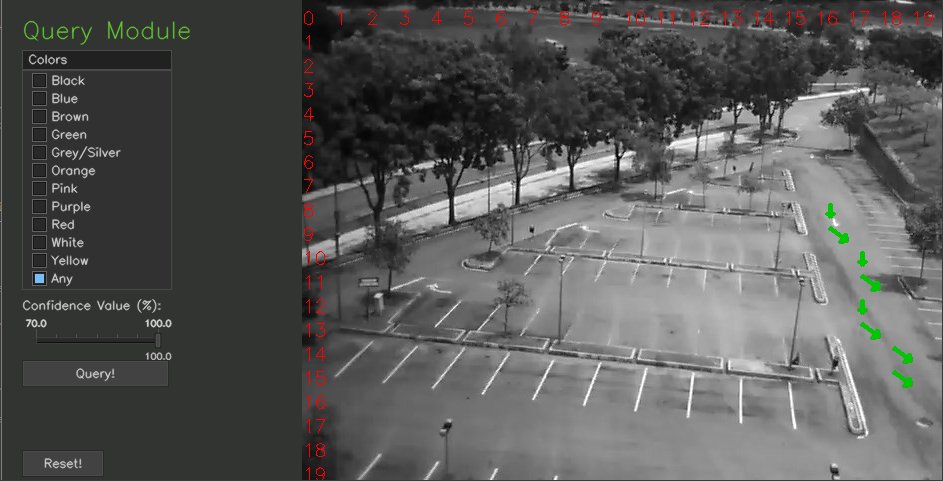
\includegraphics[width=0.7\linewidth]{image/retrievalOne/test1-8inputs.PNG} \\  
		(a) Motion Test Case 1 (TQ1) \\
		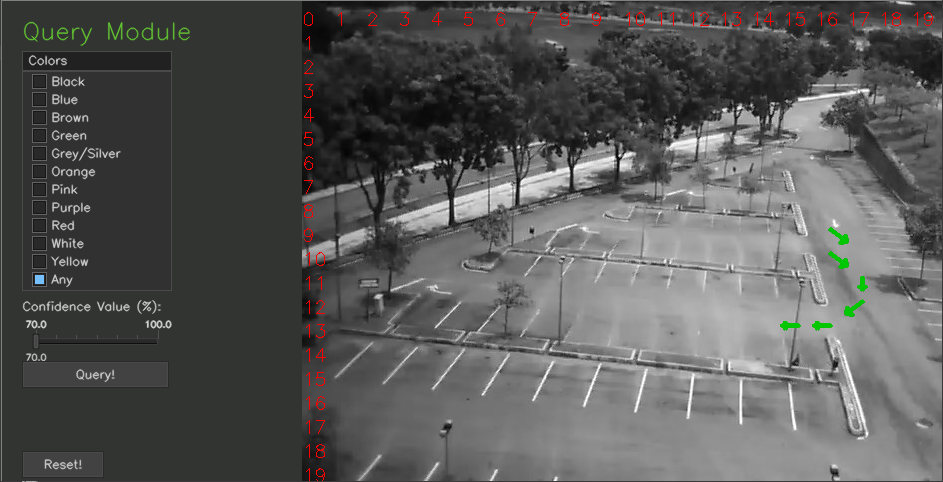
\includegraphics[width=0.7\linewidth]{image/retrievalOne/test2-6input.PNG}\\
		(b) Motion Test Case 2 (TQ2)
	\end{tabular}
	\caption{Search interface for \versionOne} 
	\label{fig:versionOneInterface}
\end{figure}




\subsection{Results}
The following subsections describes the evaluation process of the proposed method in Section \ref{section:semantic_lsh} which includes both the vehicle trajectory as well as the vehicle color.    \cc{etc}


\subsubsection{Vehicle Trajectory}
\subsubsection{Vehicle Color}

\begin{table}[bht!]
\centering
\caption{Ground truth distribution vehicle colors ordered by occurrence}
\label{table:colorDist}
\begin{tabular}{ccc}
\toprule
Color Term & No. of Occurrence & Percentage (\%)   \\
\midrule
Gray       & 365       & 43.61  \\
Black      & 182       & 21.74  \\
White      & 150       & 17.92  \\
Red        & 60        & 7.17   \\
Blue       & 19        & 2.27   \\
Orange     & 15        & 1.79   \\
Yellow     & 13        & 1.55   \\
Green      & 10        & 1.19   \\
Pink       & 9         & 1.08   \\
Purple     & 7         & 0.84   \\
Brown      & 7         & 0.84   \\
\bottomrule
\end{tabular}
\end{table}


Table \ref{table:colorMatrix} reports the confusion matrix of the color retrieval task. 
%While most of the color terms were extracted correctly \ian{this is not true, e.g. Black retrieved as Gray is 48 ... btw, is the word "predicted color" the correct term?  "deduced"?}, 
The overall precision stands at 54\%, with a recall of 36\% and $F_1$ score of 39\%. The cells in Table \ref{table:colorMatrix} marked in green indicate the highest count of correctly predicted colors, while the cells marked in red indicate the highest count of incorrect predictions for each color. Our method is able to predict correctly a majority of cases for seven out of eleven colors.

Based on the obtained results, we learn that the $T_{pivot}$ needs to be adjusted as too many chromatic vehicles were classified as achromatic vehicles which in turned affected the overall performance of the proposed method. We hypothesize that better results can be obtained by careful adjustment of $T_{pivot}$ or attempt to learn a suitable color model as in \cite{hu2015vehicle,rachmadi2015vehicle} for this particular scene. We observe that vehicles with lighter and darker shades were particularly difficult as they do not contain enough chromatic hues to arrive at a correct prediction.  

While the classification of achromatic versus chromatic vehicles faced considerable difficulties, the black \& white filters provide a considerably good result when determining the different categories of achromatic vehicles which may be useful for processing in grayscale. Based on our observation, most errors usually occur when the vehicles are in locations where the intensity of shadows overpowered the lighter-shade vehicles in terms of coverage area. 

\begin{table}[]
\centering
\caption{Confusion matrix for color retrieval task}
\vspace{1.5em}
\label{table:colorMatrix}
\resizebox{\columnwidth}{!}{
\begin{tabular}{ccccccccccccc}
\cline{3-13}
                                                      & \multicolumn{1}{l|}{}          & \multicolumn{11}{c|}{Predicted Color}                                                                                                                                                                                                                                                                                                                                                                                                                                                                                                                                                                                                                             \\ \cline{3-13} 
                                                      & \multicolumn{1}{c|}{}          & \multicolumn{1}{c|}{Gray}                                 & \multicolumn{1}{c|}{Black}                                & \multicolumn{1}{c|}{White}                                & \multicolumn{1}{c|}{Red}                                & \multicolumn{1}{c|}{Blue}                               & \multicolumn{1}{c|}{Orange}                             & \multicolumn{1}{c|}{Yellow}                             & \multicolumn{1}{c|}{Green}                              & \multicolumn{1}{c|}{Pink}                               & \multicolumn{1}{c|}{Purple}                             & \multicolumn{1}{c|}{Brown}                              \\ \hline
\multicolumn{1}{|l|}{}                                & \multicolumn{1}{c|}{Gray}      & \multicolumn{1}{c|}{\cellcolor[HTML]{32CB00}\textbf{236}} & \multicolumn{1}{c|}{61}                                   & \multicolumn{1}{c|}{68}                                   & \multicolumn{1}{c|}{0}                                  & \multicolumn{1}{c|}{0}                                  & \multicolumn{1}{c|}{0}                                  & \multicolumn{1}{c|}{0}                                  & \multicolumn{1}{c|}{0}                                  & \multicolumn{1}{c|}{0}                                  & \multicolumn{1}{c|}{0}                                  & \multicolumn{1}{c|}{0}                                  \\ \cline{2-13} 
\multicolumn{1}{|l|}{}                                & \multicolumn{1}{c|}{Black}     & \multicolumn{1}{c|}{48}                                   & \multicolumn{1}{c|}{\cellcolor[HTML]{32CB00}\textbf{134}} & \multicolumn{1}{c|}{0}                                    & \multicolumn{1}{c|}{0}                                  & \multicolumn{1}{c|}{0}                                  & \multicolumn{1}{c|}{0}                                  & \multicolumn{1}{c|}{0}                                  & \multicolumn{1}{c|}{0}                                  & \multicolumn{1}{c|}{0}                                  & \multicolumn{1}{c|}{0}                                  & \multicolumn{1}{c|}{0}                                  \\ \cline{2-13} 
\multicolumn{1}{|l|}{}                                & \multicolumn{1}{c|}{White}     & \multicolumn{1}{c|}{26}                                   & \multicolumn{1}{c|}{4}                                    & \multicolumn{1}{c|}{\cellcolor[HTML]{32CB00}\textbf{120}} & \multicolumn{1}{c|}{0}                                  & \multicolumn{1}{c|}{0}                                  & \multicolumn{1}{c|}{0}                                  & \multicolumn{1}{c|}{0}                                  & \multicolumn{1}{c|}{0}                                  & \multicolumn{1}{c|}{0}                                  & \multicolumn{1}{c|}{0}                                  & \multicolumn{1}{c|}{0}                                  \\ \cline{2-13} 
\multicolumn{1}{|l|}{}                                & \multicolumn{1}{c|}{Red}       & \multicolumn{1}{c|}{27}                                   & \multicolumn{1}{c|}{25}                                   & \multicolumn{1}{c|}{0}                                    & \multicolumn{1}{c|}{2}                                  & \multicolumn{1}{c|}{0}                                  & \multicolumn{1}{c|}{0}                                  & \multicolumn{1}{c|}{0}                                  & \multicolumn{1}{c|}{0}                                  & \multicolumn{1}{c|}{4}                                  & \multicolumn{1}{c|}{\cellcolor[HTML]{FE0000}\textbf{2}} & \multicolumn{1}{c|}{0}                                  \\ \cline{2-13} 
\multicolumn{1}{|l|}{}                                & \multicolumn{1}{c|}{Blue}      & \multicolumn{1}{c|}{3}                                    & \multicolumn{1}{c|}{10}                                   & \multicolumn{1}{c|}{0}                                    & \multicolumn{1}{c|}{0}                                  & \multicolumn{1}{c|}{\cellcolor[HTML]{32CB00}\textbf{6}} & \multicolumn{1}{c|}{0}                                  & \multicolumn{1}{c|}{0}                                  & \multicolumn{1}{c|}{0}                                  & \multicolumn{1}{c|}{0}                                  & \multicolumn{1}{c|}{0}                                  & \multicolumn{1}{c|}{0}                                  \\ \cline{2-13} 
\multicolumn{1}{|l|}{}                                & \multicolumn{1}{c|}{Orange}    & \multicolumn{1}{c|}{8}                                    & \multicolumn{1}{c|}{3}                                    & \multicolumn{1}{c|}{0}                                    & \multicolumn{1}{c|}{0}                                  & \multicolumn{1}{c|}{0}                                  & \multicolumn{1}{c|}{\cellcolor[HTML]{32CB00}\textbf{3}} & \multicolumn{1}{c|}{0}                                  & \multicolumn{1}{c|}{0}                                  & \multicolumn{1}{c|}{0}                                  & \multicolumn{1}{c|}{1}                                  & \multicolumn{1}{c|}{0}                                  \\ \cline{2-13} 
\multicolumn{1}{|l|}{}                                & \multicolumn{1}{c|}{Yellow}    & \multicolumn{1}{c|}{3}                                    & \multicolumn{1}{c|}{1}                                    & \multicolumn{1}{c|}{2}                                    & \multicolumn{1}{c|}{0}                                  & \multicolumn{1}{c|}{0}                                  & \multicolumn{1}{c|}{0}                                  & \multicolumn{1}{c|}{\cellcolor[HTML]{32CB00}\textbf{7}} & \multicolumn{1}{c|}{0}                                  & \multicolumn{1}{c|}{0}                                  & \multicolumn{1}{c|}{0}                                  & \multicolumn{1}{c|}{0}                                  \\ \cline{2-13} 
\multicolumn{1}{|l|}{}                                & \multicolumn{1}{c|}{Green}     & \multicolumn{1}{c|}{5}                                    & \multicolumn{1}{c|}{1}                                    & \multicolumn{1}{c|}{4}                                    & \multicolumn{1}{c|}{0}                                  & \multicolumn{1}{c|}{0}                                  & \multicolumn{1}{c|}{0}                                  & \multicolumn{1}{c|}{0}                                  & \multicolumn{1}{c|}{\cellcolor[HTML]{C0C0C0}\textbf{0}} & \multicolumn{1}{c|}{0}                                  & \multicolumn{1}{c|}{0}                                  & \multicolumn{1}{c|}{0}                                  \\ \cline{2-13} 
\multicolumn{1}{|l|}{}                                & \multicolumn{1}{c|}{Pink}      & \multicolumn{1}{c|}{1}                                    & \multicolumn{1}{c|}{0}                                    & \multicolumn{1}{c|}{0}                                    & \multicolumn{1}{c|}{\cellcolor[HTML]{FE0000}\textbf{3}} & \multicolumn{1}{c|}{0}                                  & \multicolumn{1}{c|}{0}                                  & \multicolumn{1}{c|}{0}                                  & \multicolumn{1}{c|}{0}                                  & \multicolumn{1}{c|}{\cellcolor[HTML]{32CB00}\textbf{5}} & \multicolumn{1}{c|}{0}                                  & \multicolumn{1}{c|}{0}                                  \\ \cline{2-13} 
\multicolumn{1}{|l|}{}                                & \multicolumn{1}{c|}{Purple}    & \multicolumn{1}{c|}{3}                                    & \multicolumn{1}{c|}{3}                                    & \multicolumn{1}{c|}{0}                                    & \multicolumn{1}{c|}{0}                                  & \multicolumn{1}{c|}{0}                                  & \multicolumn{1}{c|}{0}                                  & \multicolumn{1}{c|}{0}                                  & \multicolumn{1}{c|}{0}                                  & \multicolumn{1}{c|}{0}                                  & \multicolumn{1}{c|}{1}                                  & \multicolumn{1}{c|}{0}                                  \\ \cline{2-13} 
\multicolumn{1}{|l|}{\multirow{-11}{*}{\rotatebox[origin=c]{90}{Actual Color}}} & \multicolumn{1}{c|}{Brown}     & \multicolumn{1}{c|}{3}                                    & \multicolumn{1}{c|}{4}                                    & \multicolumn{1}{c|}{0}                                    & \multicolumn{1}{c|}{0}                                  & \multicolumn{1}{c|}{0}                                  & \multicolumn{1}{c|}{0}                                  & \multicolumn{1}{c|}{0}                                  & \multicolumn{1}{c|}{0}                                  & \multicolumn{1}{c|}{0}                                  & \multicolumn{1}{c|}{0}                                  & \multicolumn{1}{c|}{\cellcolor[HTML]{C0C0C0}\textbf{0}} \\ \hline
                                                      & \multicolumn{1}{l}{}           & \multicolumn{1}{l}{}                                      & \multicolumn{1}{l}{}                                      & \multicolumn{1}{l}{}                                      & \multicolumn{1}{l}{}                                    & \multicolumn{1}{l}{}                                    & \multicolumn{1}{l}{}                                    & \multicolumn{1}{l}{}                                    & \multicolumn{1}{l}{}                                    & \multicolumn{1}{l}{}                                    & \multicolumn{1}{l}{}                                    & \multicolumn{1}{l}{}                                    \\ \hline
\multicolumn{1}{|l|}{}                                & \multicolumn{1}{c|}{Precision} & \multicolumn{1}{c|}{65.01}                                & \multicolumn{1}{c|}{54.47}                                & \multicolumn{1}{c|}{61.86}                                & \multicolumn{1}{c|}{40.00}                              & \multicolumn{1}{c|}{100.00}                             & \multicolumn{1}{c|}{100.00}                             & \multicolumn{1}{c|}{100.00}                             & \multicolumn{1}{c|}{N/A}                                & \multicolumn{1}{c|}{55.56}                              & \multicolumn{1}{c|}{25.00}                              & \multicolumn{1}{c|}{N/A}                                \\ \cline{2-13} 
\multicolumn{1}{|l|}{}                                & \multicolumn{1}{c|}{Recall}    & \multicolumn{1}{c|}{64.66}                                & \multicolumn{1}{c|}{73.63}                                & \multicolumn{1}{c|}{80.00}                                & \multicolumn{1}{c|}{3.33}                               & \multicolumn{1}{c|}{31.58}                              & \multicolumn{1}{c|}{20.00}                              & \multicolumn{1}{c|}{53.85}                              & \multicolumn{1}{c|}{0.00}                               & \multicolumn{1}{c|}{55.56}                              & \multicolumn{1}{c|}{14.29}                              & \multicolumn{1}{c|}{0.00}                               \\ \cline{2-13} 
\multicolumn{1}{|l|}{\multirow{-3}{*}{\rotatebox[origin=c]{90}{Result}}}        & \multicolumn{1}{c|}{F1 Score}  & \multicolumn{1}{c|}{64.84}                                & \multicolumn{1}{c|}{62.62}                                & \multicolumn{1}{c|}{69.77}                                & \multicolumn{1}{c|}{6.15}                               & \multicolumn{1}{c|}{48.00}                              & \multicolumn{1}{c|}{33.33}                              & \multicolumn{1}{c|}{70.00}                              & \multicolumn{1}{c|}{N/A}                                & \multicolumn{1}{c|}{55.56}                              & \multicolumn{1}{c|}{18.18}                              & \multicolumn{1}{c|}{N/A}                                \\ \hline
\end{tabular}%
}
\end{table}


% However, the current implementation of the proposed method search interface has yet to include time slicing query options. 

% js: don't quite understand this
%However, should the initial test against the $T_{pivot}$ fails, the proposed method is able to fall back on the HSV histogram results.


\section{\versionTwo}

\subsection{Concept}

Contrary to the proposed interface in \versionOne which is written in C++, this interface here is written in javascript which can be easily extendable to web interfaces.

\subsection{Scoring System}
\subsection{Vehicle Trajectory}
\subsection{Vehicle Color \& Color Mode}
\subsection{Results}

\section{Result Analysis}
We also note that the achromatic algorithm is an essential step because the 8 Values bins are insufficient to accurately represent vehicles with borderline dominant color as the brightness values may be widely distributed.



\cc{for the analysis, include a "heatmap" of the versionone vs versiontwo for the evaluation of results}


